\chapter{Combining models}\label{ch:03}

\begin{chapter_outline}

  In this chapter, we demonstrate the benefits of combining distinct class of models with a concrete example. In particular, we study the complementary of variational autoencoders (VAEs) and denoising diffusion probabilistic models (DDPMs). VAEs offer scalable amortized posterior inference and fast sampling but are also more and more outperformed by competing models such as normalizing flows (NFs) or deep-energy models. We improve VAEs by modelling the prior distribution of the latent variables with a diffusion process. The diffusion prior model improves upon Gaussian priors of classical VAEs and is competitive with NF-based priors.
  This contribution shows that connecting different classes of deep probabilistic models can unlock new modelling capacity and properties that are unreachable by each class of models independently.
\end{chapter_outline}
\section{Prologue}
In this chapter we bring evidence to argue that different (deep) probabilistic models shall not be studied independently. Building a broad understanding of all these frameworks unlocks a large number of model combinations. These combinations help to reduce the weaknesses of each class of models separately while maintaining the separate assets of each class.

The gradient-descent-based training framework of neural networks is key in the development of `super` deep probabilistic models that combines together more than one type of models. This strategy allows learning all components of a `super` model jointly as soon as we express the final objective as a differentiable function of these components. In this chapter, we take advantage of this feature to combine denoising diffusion probabilistic models and variational autoencoders.

As will see in the paper, combining DDPMs and VAEs is fairly straighforward and leads to better modelling for image synthesis. We believe that fostering further the interplay between different probabilistic models is important in the development of the probabilistic modelling toolbox. In an ideal world, combining two classes of deep probabilistic models should be as simple as replacing a Normal distribution by a Laplace distribution in a probabilistic program. Building this ideal world should eventually help practicioners to define models with all the key properties required for their final application.

\section{The paper: Diffusion Priors In Variational Autoencoders}

\subsection{Author contributions}
The paper is co-authored by me and Gilles Louppe. As the leading author, I developed the connections between diffusion models and variational autoencoders, made the experiments, and wrote the paper. In particular, I derived the ELBO associated to the denoising diffusion priors in VAES. Gilles Louppe supervised me throughout this project, offered suggestions and helped in writing the paper.

\subsection{Reading tips}
The reader may skip section 2 which presents VAEs and DDPMs already introduced the background chapter. The reader interested in deeply understanding the implementation of DDPMs should take a look at \citet{ho_denoising_2020}. The rest of the paper should flow naturally.

\subsection{Minor corrections}
There is a missing negative sign in Equation~(20) which becomes
$$\mathcal{L}(\mathbf{x}; \phi, \theta, \psi) := -\mathbb{E}_{q_{\psi}}\left[\log \frac{p_{\mathbf{\theta}}(\mathbf{x}|\mathbf{z})}{q_{\psi}(\mathbf{z}|\mathbf{x})} \right] + \mathbb{E}_{q_{\psi}}\left[ L_{\text{DDPM}}(\mathbf{z}_0; \phi)\right].$$

\includepdf[pages=-]{papers/innf_latent_diffusion.pdf}

\section{Epilogue}

Our initial motivation for combining diffusion models and VAEs was not to improve VAEs. Instead, we wanted to enable new types of noise for training diffusion models. Intuitively, the noise model provides an inductive bias to the learning algorithm, and adapting the noise to the data modality might help learn a better generative model. In particular, we thought heat equations would provide an appealing inductive bias for image synthesis. Heat equation blurs the image along time; it corresponds to first discarding information about the details of the image and removing the semantic content only later in the noising process.

Our idea was to use a VAE formulation to bypass the closed-form gaussian kernel required for obtaining a tractable training objective. In addition, we thought playing with different diffusion speeds inside the latent variables of the VAE would eventually enforce different levels of structure between latent variables with varying schedules of diffusion. This would have provided an elegant way of extracting high and low-level semantic information from images and creating exciting applications based on conditional generative modelling.

Unfortunately, I did not figure out a good training algorithm for these models. Recently, \citet{rissanen2022generative} had a similar idea and achieved state-of-the-art image synthesis with a diffusion model based on the heat equation instead of the diffusion equation. In the future, it would be interesting to combine heat diffusion with VAEs to compress data into human-interpretable latent variables representing high and low-level features.

\subsection{Scientific impact}

According to Google Scholar, our article has received five citations between its publication in June 2021 and July 2022. It is interesting to contrast this number with the 48 citations received by \citet{vahdat2021score}, which was published in December 2021 at NeurIPS 2021 and was first released as a preprint on Arxiv in June 2021. Although the ideas expressed in the two papers are similar, our work did not gain as much visibility as theirs. We acknowledge at least three \textbf{fair} reasons to explain this. First, publishing at NeurIPS brings much more visibility than at a workshop at ICML. This is natural as the reviewing process of NeurIPS is much stronger. Second, \citet{vahdat2021score} achieve state-of-the-art image synthesis by combining their idea with the proper neural architectures, training tricks and computation power.
In contrast to theirs, our work is more preliminary as it does not achieve state-of-the-art performance. Finally, advertising science is arguably nowadays as important as the science itself in machine learning.\citet{vahdat2021score} made an excellent job, as can be seen by one tweet from the first author who advertised their paper in \Cref{fig:cont_tweet} and had $6\times$ higher reach than a similar advertisement by Gilles Louppe in \Cref{fig:discrete_tweet}.

\subsection{Conclusion and opportunities}
Since the publication of this article, diffusion models have become very popular, owing part of their success to the astonishing results achieved by large text-to-images models created by OpenAI~\citep[$\text{DALL}\cdot\text{E} 2$][]{ramesh2022hierarchical} and Google~\citep[Imagen][]{saharia2022photorealistic}. Close to our work, \citet{yu2022latent} recently proposed to use energy based models trained with denoising score matching to model the prior distribution of VAEs for interpretable text modelling. In the close future, the attractivity of diffusion models for modelling distributions over images, and potentially other data modalities, should stay high. Their remain many open questions about why these models are able to represent high dimensional data such as images so well. The main drawbacks of diffusion is the sampling procedure which is not direct and requires to perform many denoising steps. Pushing further the connections between diffusion models and other probabilistic models such as normalizing flows and VAEs might help in reducing the complexity of sample synthesis.

\begin{figure*}
  \centering
  \begin{subfigure}[b]{.48\textwidth}
    \centering
    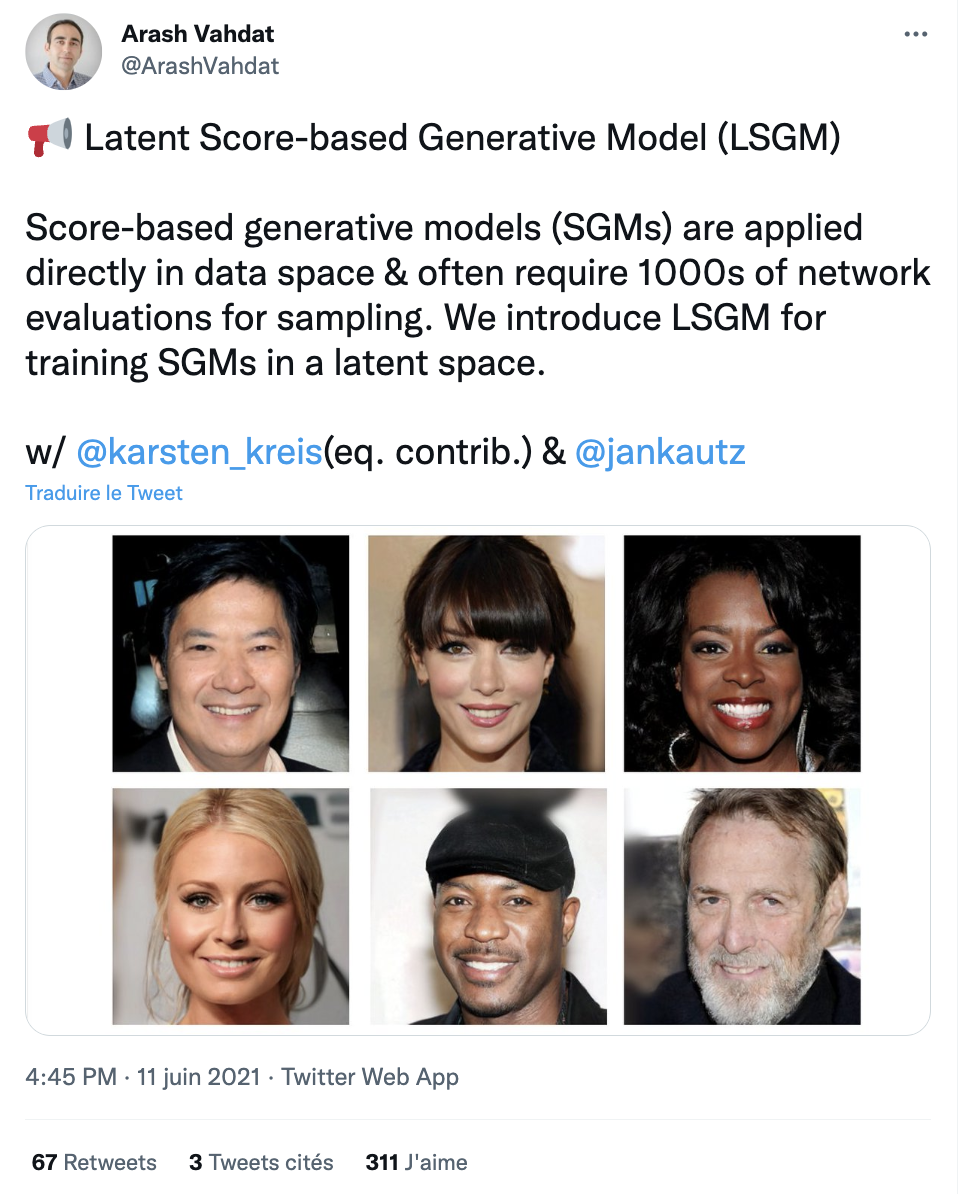
\includegraphics[width=.95\textwidth]{figures/impact_scholar/cont_diff_tweet.png}
    \caption{}
    \label{fig:cont_tweet}
  \end{subfigure}
  \begin{subfigure}[b]{.48\textwidth}
    \centering
    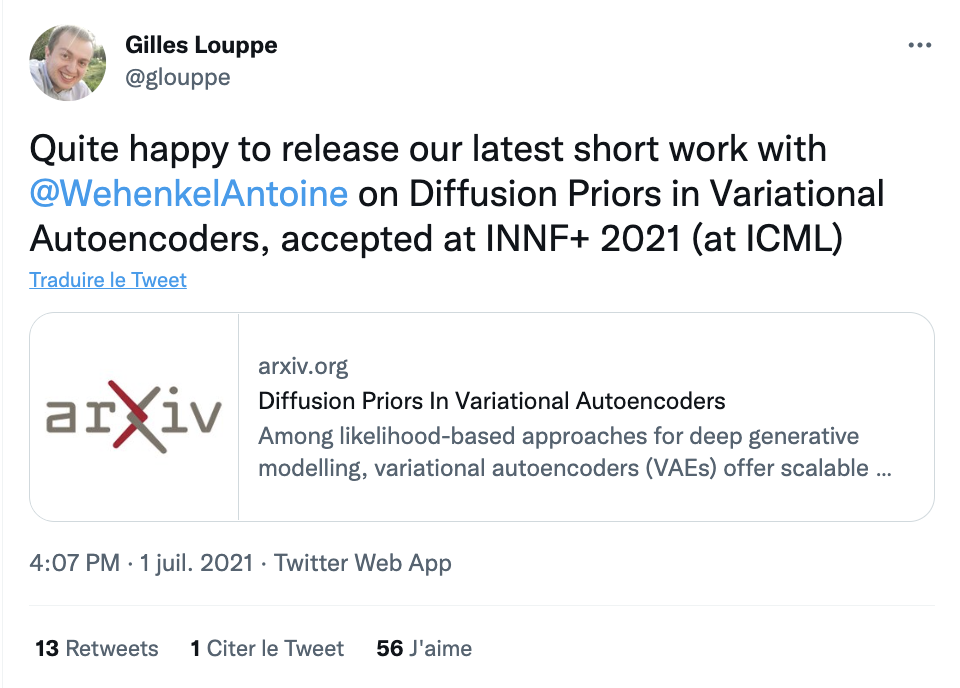
\includegraphics[width=.95\textwidth]{figures/impact_scholar/discret_diff_tweet.png}
    \caption{}
    \label{fig:discrete_tweet}
  \end{subfigure}
  \caption{Tweets advertising (\textbf{a}) The continuous-time diffusion models in the latent space from \citet{vahdat2021score} (\textbf{b}) The discrete-time diffusion models in the latent space from ours.}
\end{figure*}
